\chapter{Desarrollo del proyecto}
\label{cap:estadodelarte}


\section{Antecedentes de la empresa}

\subsection{Descripción de la empresa}

3Dlux es un emprendimiento dedicado al diseño e impresión 3D, fundada el año 2016 por Javier Oliva y Juan Marinetti. La empresa comenzó con el propósito de utilizar la tecnología de impresión 3D FDM para la fabricación de piezas, enfocadas principalmente a las soluciones del área industrial y manufactura. Así, el año 2017 la empresa comenzó con una etapa de investigación y aprendizaje de la maquinaria para estos efectos, y la posibles industrias en las cuales la impresión 3D podría agregar valor. El interés de Javier, diseñador de profesión, por trabajar con softwares de diseño 3D y la visión de Juan, empresario, por incursionar en nuevas áreas de negocio, fueron dando forma al estado actual de la empresa. 
La primera capacitación o acercamiento a la industria fue en Estados Unidos, donde Javier estuvo de pasante en la empresa de impresión 3D \textit{3DChimera} durante dos semanas. Tanto las máquinas como el modelo de negocio que utilizaban, fueron tomados como ejemplo para lo que se implementaría en Chile. Posterior a este hecho, el primer año de desarrollo se llevó a cabo con la colaboración de la empresa \textit{Acrus-ccl}, dedicada al etiquetado de vinos ubicada en la comuna de Conchalí. Allí, haciendo uso de una oficina facilitada para estos efectos, se instalaron las primeras máquinas e impresoras 3d, haciendo trabajos ocasionales y a pedido. En 2018, la empresa se trasladó a las dependencias de la Fundacion Mustakis, en la comuna de Recoleta, emplazamiento que ocupa en la actualidad. Hoy, el taller cuenta con 9 impresoras 3d y desarrolla piezas para distintas industrias como minería, salud, entre otras. La capacidad instalada ha permitido la producción de piezas de un volumen aproximado de 300 unidades por pedido; asimismo, la diversidad de impresoras da la posibilidad de trabajar con diversos filamentos de impresión 3D, tanto materiales tradicionales (PLA, ABS y PETG) como plásticos de ingeniería (ASA, PC, entre otros). Dentro de los servicios ofrecidos está el diseño y fabricación de productos y piezas, escaneo 3D y capacitaciones orientadas al uso de las máquinas. 

\subsection{Proceso de impresión 3D}

El proceso de impresión 3D, a grandes rasgos, consiste en:

\begin{itemize}
\item Exportación de la pieza a lenguaje estándar de triángulos (.stl).
\item Configuración de variables de impresión en software CAM.
\item Exportación de la pieza en formato .gcode.
\item Carga de archivo en la máquina.
\item Precalentamiento de la máquina.
\item Fabricación de la pieza.
\item Extracción de la pieza y post-proceso en caso de ser necesario.
\end{itemize}

El diagrama de flujo que representa el proceso, decisiones y resultados, se muestra a continuación:

\begin{figure}[H]
\centering

\includegraphics[scale=0.4]{images/proceso.png}
\caption{Diagrama de flujo del proceso de impresión 3D.}
\end{figure}


\section{Descripción del Problema}

Las ventajas del proceso de impresión 3D FDM como la fabricación de diseños complejos, el bajo coste de inversión y la obtención de un objeto final, han hecho que muchas empresas dedicadas al rubro de la manufactura comiencen a incorporar a sus lineas estas máquinas. Por otra parte, la existencia de pequeñas empresas y emprendimientos dedicados a la impresión 3D ha generado un avance en el conocimiento, aplicación y difusión de esta tecnología. Sumado a lo anterior, la personalización de los productos en masa da lugar a que, para maximizar la producción, es necesario el control y la gestión de una mayor cantidad de impresoras. Es por esto que, a mayor cantidad de máquinas, también aumenta la complejidad, ya sea en la operación misma, o mantenerlas en un estado confiable y disponible. A medida que fue aumentando la cantidad de activos, la empresa se vio en la necesidad de optimizar el proceso de producción y mantenimiento, detectando los siguientes problemas:

\begin{itemize}
\item Imposibilidad de monitorización de múltiples máquinas funcionando a la vez.
\item Impresoras detenidas frecuentemente por mantenimiento correctivo.
\item Impresoras detenidas por varias horas debido a dificultades con la identificación de los problemas.
\item Existencia nula o insuficiente de datos referidos a los mantenimientos realizados.
\item Existencia nula o insuficiente de datos referidos al material utilizado.
\end{itemize}





\section{ Aplicación de mantenimiento basado en la teoría de la confiabilidad}


\subsection{Selección del equipo}

El primer paso para determinar la máquina de impresión 3D más crítica, es la realización de un análisis de criticidad a los equipos del taller. Debido a que la empresa no ha registrado periódicamente las fallas ocurridas y las acciones de mantenimiento realizadas, el análisis se basará en establecer cual sería la condición más favorable, así como la condición menos favorable de cada uno de los criterios a evaluar, según apreciaciones generales e información obtenida en los últimos seis meses. Para esto, los aspectos a evaluar son:

\begin{itemize}
\item Impacto a la seguridad
\item Costo de reparación
\item Frecuencia de las fallas
\item Costo operacional
\end{itemize}

Las tablas de ponderaciones para cada uno de estos son las siguientes:

\begin{table}[H]
  \centering
  
    \begin{tabular}{|l|r|}
    \hline
    Frecuencia de las fallas & \multicolumn{1}{l|}{Ponderación} \\
    \hline
    mayor que 16 /semestre & 5 \\
    \hline
    12-15/semestre & 4 \\
    \hline
    8-11/semestre & 3 \\
    \hline
    4-7/semestre & 2 \\
    \hline
    Menor a 4/al semestre & 1 \\
    \hline
    \end{tabular}%
    \caption{Ponderaciones para el ítem de frecuencia de fallas}
  \label{tab:addlabel}%
\end{table}%

\qquad\qquad%

\begin{table}[H]
  \centering
 
    \begin{tabular}{|l|r|}
    \hline
    Costo de reparación & \multicolumn{1}{l|}{Ponderación} \\
    \hline
    mayor a \$80.000 & 10 \\
    \hline
    \$60.000 - \$79.000 & 8 \\
    \hline
    \$40.000 - \$59.000 & 6 \\
    \hline
    \$20.000 - \$39.000 & 4 \\
    \hline
    Menor a \$20.000 & 2 \\
    \hline
    \end{tabular}%
    \caption{Ponderaciones para el ítem de costo de reparación}
  \label{tab:addlabel}%
\end{table}%

\begin{table}[H]
  \centering
 
    \begin{tabular}{|l|r|}
    \hline
    Impacto a la seguridad & \multicolumn{1}{l|}{Ponderación} \\
    \hline
    Muy grave & 10 \\
    \hline
    Grave & 8 \\
    \hline
    Severo  & 6 \\
    \hline
    Moderado & 4 \\
    \hline
    Bajo  & 2 \\
    \hline
    \end{tabular}%
    \caption{Ponderaciones para el ítem de Impacto a la seguridad}
  \label{tab:addlabel}%
\end{table}%

\begin{table}[H]
  \centering
  
    \begin{tabular}{|l|r|}
    \hline
    Impacto Operacional & \multicolumn{1}{l|}{Ponderación } \\
    \hline
    Para la operación & 15 \\
    \hline
    80\% de parada & 12 \\
    \hline
    60\% de parada & 9 \\
    \hline
    40\% de parada & 6 \\
    \hline
    20\% de parada & 3 \\
    \hline
    \end{tabular}%
    \caption{Ponderaciones para el ítem de impacto operacional}
  \label{tab:addlabel}%
\end{table}%

Los resultados del análisis de criticidad para elegir el activo más crítico se muestran en la siguiente tabla:

\begin{table}[H]
  \centering
  
    \begin{tabular}{|r|p{2cm}|p{1cm}|p{1cm}|p{1cm}|p{1cm}|p{1cm}|p{1cm}|}
    \hline
    \multicolumn{1}{|l|}{Ítem} & Activo & \multicolumn{1}{p{1.5cm}|}{Frecuencia de fallas} & \multicolumn{1}{p{1.5cm}|}{Seguridad} & \multicolumn{1}{p{1.5cm}|}{Operacional} & \multicolumn{1}{p{1.5cm}|}{Reparación} & \multicolumn{1}{p{1cm}|}{Total Consec.} & \multicolumn{1}{p{1cm}|}{Critic. Total} \\
    \hline
    1     & Impresora PRUSA MK3 & 1 & 2& 9 & 8& 19& 19 \\
    \hline
    2     & Impresora ENDER 3 & 1  & 2 & 6 & 4 & 12 & 12 \\
    \hline
    3     & Impresora X350 G. RepRap & 3& 4 & 12 & 8  & 24 & 72 \\
    \hline
    4     & Impresora X400 G. RepRap & 2 & 4 & 12 & 8 & 24 & 48 \\
    \hline
    \end{tabular}%
    \caption{Análisis de criticidad para determinar el activo más crítico.}
  \label{tab:addlabel}%
\end{table}%

El puntaje final se obtiene multiplicando el valor obtenido de las frecuencias por la sumatoria total de las consecuencias para cada Activo. De este análisis se desprende que la impresora \textit{X350 German RepRap} es el equipo con mayor criticidad en función de las variables estudiadas, en el periodo comprendido por seis meses desde marzo hasta agosto del 2020.

\subsection{Descripción del equipo}

La máquina modelo X350 de la fundación GermanRepRap es una impresora 3D de código abierto, dirigida tanto a consumidores en general como a usuarios industriales. Posee un cabezal de doble extrusión, superficie de construcción rectangular descendente con respecto al eje-z y  climatizada. El volumen total de la máquina es de 600x444x517 mm y el volumen de construcción comprende los 350x200x210 mm.

A continuación, se resumen los datos técnicos generales de la máquina: 

\begin{table}[H]
  \centering
  
    \begin{tabular}{|l|l|}
    \hline
    Materiales & ABS, PLA, PS, PP, PVA \\
    \hline
    Dimensiones & 600x444x517 mm \\
    \hline
    Volumen de impresión & 350x200x210 mm \\
    \hline
    Voltaje de Operación & 110/230 V \\
    \hline
    Consumo & 250 W \\
    \hline
    Configuración  & Unidad prefabricada/Lista para imprimir \\
    \hline
    Tecnología & FDM \\
    \hline
    Grosor de capa & 0,02 mm \\
    \hline
    Velocidad de impresión  & 10-150 mm/s \\
    \hline
    Velocidad de viaje & 10-300 mm/s \\
    \hline
    Cama de impresión & T° max 120°C \\
    \hline
    Conexión a red & WLAN/Ethernet \\
    \hline
    Peso  & 29 Kg \\
    \hline
    Boquilla & 0,4 mm \\
    \hline
    \end{tabular}%
    \caption{Ficha Técnica de la máquina X350 German RepRap \citep{germanreprap2019}.}
  \label{tab:addlabel}%
\end{table}%

\begin{figure}[H]
\centering
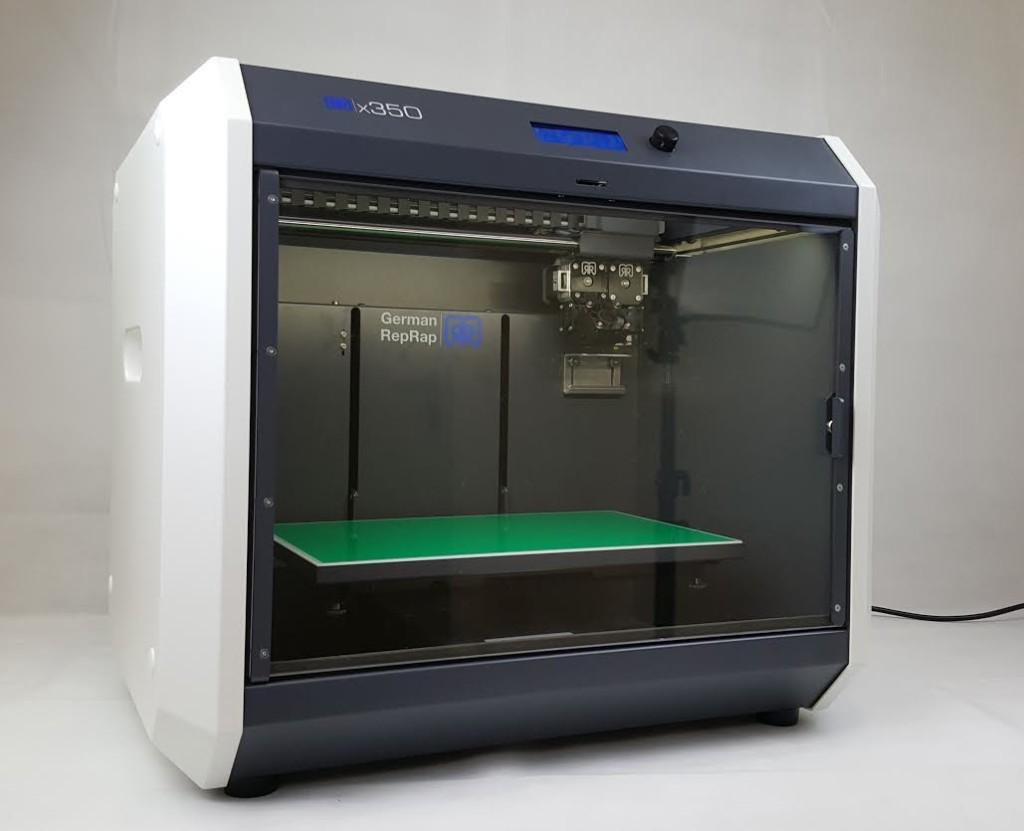
\includegraphics[scale=0.4]{images/x350pormientras.jpg}
\caption{Impresora X350.}
\end{figure}

Los componentes principales del equipo son:

\begin{itemize}
\item Paneles de chapa metálica: cubierta lateral plegada, que sirve como estructura y bancada de la máquina. Contempla el volumen completo de la impresora, y sirve como barrera térmica para el volumen de fabricación. 
\item Paneles de metacrilato: cubierta superior y barrera frontal de la máquina. Sirve como barrera térmica y está unida a la estructura de chapa metálica por medio de bisagras.
\item Varillas lisas: varillas de acero rectificadas de diámetro 8 mm, cuya función es servir de guía para los ejes del plano x-y. Las varillas del eje-x están unidas a dos carros laterales; las varillas del eje-y están unidas a la estructura de panel de chapa metálica, y soportan los carros del eje-x.
\item Rodamientos lineales: elementos de rodadura para el movimiento en el plano x-y. Están unidas, tanto a los carros del eje-y como al cabezal de impresión en el eje-x.
\item Husillos: barra roscada de diámetro 8 mm y paso 2 mm que sirve como elemento de transmisión de movimiento desde los motores paso a paso a la cama caliente en el eje-z. 
\item Motores Paso a Paso: dispositivo electromecánico que transforma los pulsos eléctricos a movimiento angular. Los motores paso a paso que componen la impresora son del tipo NEMA 17, con una corriente máxima de 1.5 A. Existe uno para generar el movimiento de cada eje.
\item Correas GT2: elemento de transmisión de movimiento desde los motores paso a paso a los ejes x-y. la transformación de movimiento angular a lineal se realiza en las poleas dentadas unidas al motor.
\item Cama caliente: superficie de impresión de la impresora 3D compuesta por una resistencia que abarca toda el área. 
\item Termistor: componente electrónico resistivo de 100K, que funciona como sensor de temperatura de extrusor y cama caliente.
\item Extrusor E3D: componente mecánico de empuje de filamento. Está compuesto por piezas que ejercen presión al filamento contra la rueda del motor de extrusión.
\item Difusor: Componente metálico cilíndrico construido con un número específico de aletas, que sirve como disipador térmico del conjunto extrusor.
\item Ventilador de difusor: pequeña turbomáquina que produce un flujo de aire constante contra el difusor, para enfriar de forma eficiente el conjunto extrusor.
\item Ventilador de capa: pequeña turbomáquina que produce un flujo de aire contra la capa en construcción, con el fin de solidificar el plástico apenas es extruido por la boquilla.
\item Garganta: Conducto metálico con hilos en su exterior. Está unido tanto al difusor como al bloque calentador y sirve como conducto para el paso del filamento hasta la zona de calentamiento.
\item Calentador: resistencia de material cerámico de alta potencia, que sirve como elemento calentador para fundir el filamento.
\item Bloque calentador: Bloque metálico que sirve como elemento térmico y de unión entre garganta y boquilla.
\item Boquilla: elemento fabricado en latón o acero con un diámetro de salida menor al de entrada. Es la pieza final del conjunto extrusor y entrega un flujo constante de plástico para la fabricación de la pieza.
\item Placa electrónica: Placa de circuito impreso compuesta por un microcontrolador re-programable y pines de entrada y salida. Este elemento controla la impresora en su conjunto y establece la comunicación entre el microcontrolador, los sensores y actuadores.
\item Interfaz LCD: dispositivo electrónico que muestra información relevante de la impresora en forma gráfica y sirve como elemento de interacción entre el operador y la máquina. Cuenta con una conexión para tarjetas SD, una pantalla LCD y un potenciómetro para controlar la impresora 3D. 
\item Fuente de alimentación: fuente conmutada que trasforma la energía eléctrica de corriente continua a alterna. Alimenta la placa electrónica, los dispositivos electromecánicos y resistivos de la máquina. 
\end{itemize}

A continuación, se resumen las recomendaciones de mantenimiento y los problemas frecuentes que el fabricante entrega en su guía para el usuario \citep{germanreprap2019}:

\begin{table}[H]
  \centering
 
    \begin{tabular}{|p{9.215em}|p{19.645em}|}
	\hline    
    Problema & \multicolumn{1}{l}{Solución} \\
	\hline    
    El equipo no enciende & Revise la fuente de alimentación \\
	\hline    
    El extrusor no calienta & Revise si la conexión del cable del calentador está bien conectada \\
	\hline    
    la cama no caliente & Revise si la conexión del cable de la cama está bien conectada \\
	\hline    
    La impresora se detiene en medio del proceso & Revise los siguientes ítem: Fuente de poder, tarjeta SD, Gcode inválido \\
	\hline    
    No hay material saliendo de la boquilla, o el flujo es inconsistente & Rectifique la presión de contacto en el extrusor, limpie la boquilla, revise la alimentación de filamento \\
	\hline    
    el objeto en impresión se despega de la cama & Limpie la superficie de construcción. Si es necesario, lubrique la cama con acetona. Verifique la distancia entre la boquilla y la superficie.  \\
	\hline    
    \end{tabular}%
     \caption{Tabla de problemas frecuentes entregados por el fabricante.}
  \label{tab:addlabel}%
\end{table}%


\subsection{Contexto Operacional}

El activo en cuestión realiza sus operaciones en el Taller de Impresión 3Dlux, ubicado en la calle Puma 1180, comuna de Recoleta. Durante los dos años previos a 2020, la máquina operaba junto a otras ocho máquinas impresoras 3D FDM de tipología cartesiana y diversos volúmenes de impresión. Debido al contexto de emergencia sanitaria, se determinó que existirían dos lugares para la producción, reduciendo la cantidad de máquinas en el taller a cuatro. La capacidad de producción de las máquinas se encuentra entre 50 y 80 gramos por hora, dependiendo del material utilizado y otras variables asociadas al proceso de impresión. El recinto es de 55,44 metros cuadrados (6,6x8,8m),el piso  es de carpeta de hormigón y el encielado con aislante térmico de fibra sintética. Cuenta con aislación térmica del exterior a través de muros de albañilería y termopaneles. Asimismo, presenta control de temperatura ambiente a través de una bomba de calor situada a un costado de la entrada al taller. Las máquinas de impresión 3D están situadas en una repisa con base metálica y cubierta de madera contrachapada. La alimentación eléctrica disponible consta de salidas a 220V AC.

\begin{figure}[H]
\centering
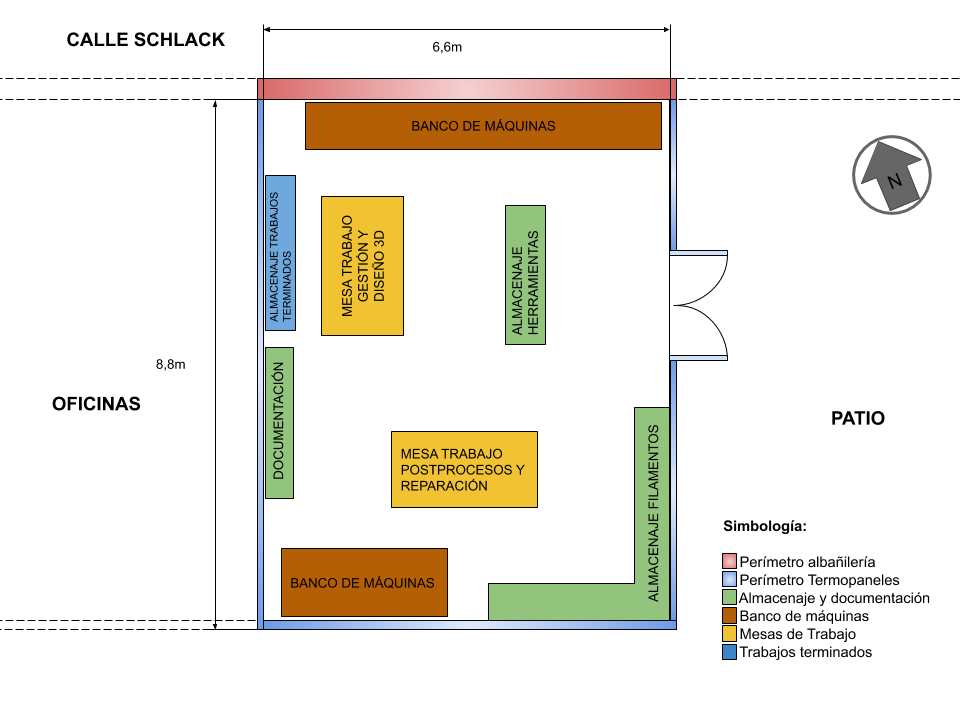
\includegraphics[scale=0.4]{images/layout.png}
\caption{Layout y simbología del taller de impresión 3D.}
\end{figure}

\subsection{Delimitación de funciones}

Para expresar de forma gráfica el funcionamiento de una impresora 3D comprendida como un sistema, se elige el diagrama funcional de bloques. Esta herramienta permite representar gráficamente el flujo de variables entre los diversos procesos de un sistema, así también sus entradas y salidas. En el diagrama mostrado a continuación, se representan las interacciones internas y externas en el sistema comprendido por la máquina. Asimismo, se observa que si una de las interacciones se ve interrumpida, quiere decir que existe algún tipo de falla en la impresora, y su efecto puede propagarse en la medida que afecte a alguno de los componentes funcionales.

\begin{figure}[H]
\centering
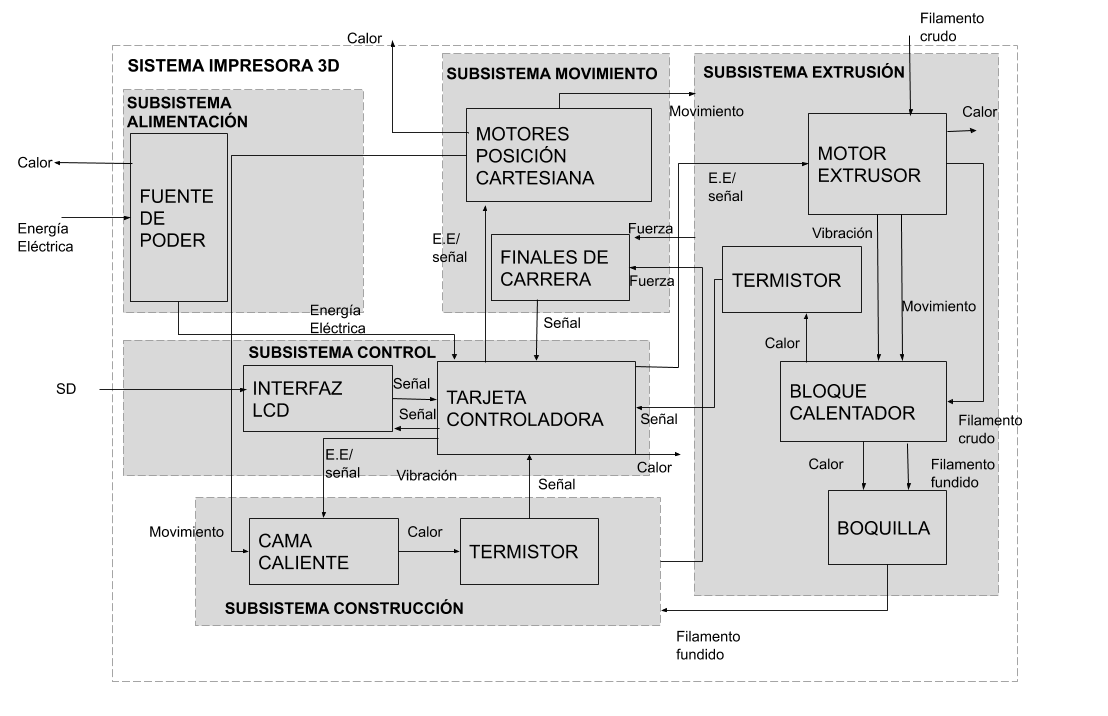
\includegraphics[scale=0.4]{images/diagramafuncional.png}
\caption{Diagrama funcional de bloques para la máquina de impresión 3D.}
\end{figure}

\subsection{Determinación de fallas}
 
Según \cite{pique1998}, el método de árbol de fallos o FTA por sus siglas en inglés \textit{Fault Tree Analysis} se trata de un método deductivo de análisis que parte de la previa selección de un suceso no deseado o evento que se pretende evitar. Seguidamente, de manera sistemática y lógica se presentan las combinaciones de las situaciones que pueden dar a lugar a la producción del evento a evitar. Se deben conformar niveles sucesivos de tal manera que cada suceso esté generado a partir de sucesos del nivel inferior siendo el nexo de unión entre los niveles la existencia de operadores o puertas lógicas \citep{pique1998}. En la siguiente tabla se muestran los símbolos que se utilizan en el árbol de falla.
 
\begin{table}[H]
\centering
\begin{tabular}{|l|p{7cm}|}
\hline
Símbolo & Significado \\
\hline

\includegraphics[scale=1]{images/arbol/basico.png} & Suceso básico. No requiere de posterior desarrollo al considerarse un suceso de fallo básico. \\ 
\hline

\includegraphics[scale=1]{images/arbol/nodesarrollado.png} & Suceso no desarrollado. No puede ser considerado como básico, pero sus causas no se desarrollan, sea por falta de información o por su poco interés.\\
\hline

\includegraphics[scale=1]{images/arbol/intermedio.png} & Resultante de la combinación de sucesos más elementales por medio de puertas lógicas. Asimismo, se representa en un rectángulo el proceso no deseado del que parte todo el árbol. \\
\hline

\includegraphics[scale=1]{images/arbol/puertay.png} & El suceso de salida ocurrirá si ocurren todos los sucesos de entrada.\\
\hline

\includegraphics[scale=1]{images/arbol/puertao.png} & El suceso de salida ocurrirá si ocurren uno o más de los suceso de entrada\\
\hline

\includegraphics[scale=1]{images/arbol/transferencia.png} & Indica que el árbol continúa en otro lugar. \\
\hline
\end{tabular}
\caption{Símbolos y significados del árbol de fallas \citep{pique1998}}
\end{table}

Según \cite{pique1998}, los pasos para la resolución de árboles de fallo son los siguientes:

\begin{enumerate}
\item Identificar todas las puertas lógicas y sucesos básicos
\item Resolución de todas las puertas en sus sucesos básicos
\item Eliminación de los sucesos repetidos en los conjuntos de fallos.
\item Eliminación de los conjuntos de fallo que contengan a su vez conjuntos de fallo más pequeños.
\end{enumerate}

\begin{figure}
\centering

\includegraphics[scale=0.4]{images/arbol/arbol1.png}
\caption{Árbol de fallas de impresora 3D.}
\end{figure}

\section{Aplicación de metodología Design Thinking para el desarrollo de Software}







